\documentclass[epsfig,10pt,fullpage]{article}

\newcommand{\LabNum}{1}
\newcommand{\CommonDocsPath}{../../../../common/docs}
\addtolength{\textwidth}{1.5in}
\addtolength{\oddsidemargin}{-0.75in}
\addtolength{\topmargin}{-0.75in}
\addtolength{\textheight}{1.5in}
\addtolength{\evensidemargin}{0.75in}
\setlength\parindent{0pt}
\raggedbottom

\usepackage{ae,aecompl}
\usepackage{epsfig,float,times}
\usepackage[hypcap]{caption}
\usepackage[pdftex, colorlinks]{hyperref}
\usepackage{graphicx}
\usepackage[usenames, dvipsnames]{color}
\usepackage{rotating}
\usepackage{tikz}
\usetikzlibrary{automata,positioning}
\usepackage{placeins}

\widowpenalty 10000
\clubpenalty 10000

\newcommand{\red}[1]{{\color{red}\sf{#1}}}
\newcommand{\green}[1]{{\color{green}\sf{#1}}}
\newcommand{\blue}[1]{{\color{blue}\sf{#1}}}
\definecolor{PineGreen}{rgb}{0.0, 0.47, 0.44}
\definecolor{ForestGreen}{rgb}{0.13, 0.55, 0.13}
\definecolor{Brown}{rgb}{0.59, 0.29, 0.0}

\newcommand{\UPDatePublished}{Oct 2021}
\newcommand{\versnum}{21.1} %version number quartus/AMP
\newcommand{\quartusname}{Quartus\textsuperscript{\textregistered} Prime}	
\newcommand{\UPTextBar}{For \quartusname{} \versnum{}}
\newcommand{\thisyear}{2021 } %for copyright
\newcommand{\company}{FPGAcademy.org}
\newcommand{\longteamname}{FPGAcademy.org}
\newcommand{\teamname}{FPGAcademy}
\newcommand{\website}{FPGAcademy.org}

\newcommand{\productAcronym}{AMP}
\newcommand{\productNameShort}{Monitor Program}

\newcommand{\productNameMedTM}{A Monitor Program}
\newcommand{\productNameMed}{A Monitor Program}

%\newcommand{\headerLogoFilePath}[1]{#1/FPGAcademy.png}

% listings is a package that supports encapsulating source code in LaTeX conveniently
\usepackage{listings}

\def\expandparam\lstinputlisting[#1]#2{\edef\tmp{\noexpand\lstinputlisting[#1]{#2}}\tmp}

%%%%%%%%%%%%%%%%%%%% Source Code Formatting %%%%%%%%%%%%%%%%%%%%
\definecolor{globalCommentColour}{rgb}{0.588,0.588,0.588}

%%%%%%%%%%%%%%%%%%%%%%%%%%%%%%%%%%%%%%%%%%%%%%%%%%%%
% Defining language style
% NiosII ASM
\lstdefinelanguage[NiosII]{Assembler} {
  morekeywords={add, addi, and, andhi, andi, beq, bge, bgeu, bgt, bgtu, ble,  bleu, blt, bltu, bne, br, break,
  bret, call, callr, cmpeq, cmpeqi, cmpge, cmpgei, cmpgeu, cmpgeui, cmpgt, cmpgti, cmpgtu, cmpgtui, cmple,
  cmplei, cmpleu, cmpleui, cmplt, cmplti, cmpltu, cmpltui, cmpne, cmpnei, custom, div, divu, eret, flushd,
  flushda, flushi, flushp, initd, initda, initi, jmp, jmpi, ldb, ldbio, ldbu, ldbuio, ldh, ldhio, ldhu, ldhuio,
  ldw, ldwio, mov, movhi, movi, movia, movui, mul, muli, mulxss, mulxsu, mulxuu, nextpc, nop, nor, or, orhi, ori,
  rdctl, rdprs, ret, rol, roli, ror, sll, slli, sra, srai, srl, srli, stb, stbio, sth, sthio, stw, stwio,
  sub, subi, sync, trap, wrctl, wrtcl, wrprs, xor, xori, xorhi, xori},
  morekeywords=[2]{.abort, .ABORT, .align, .app-file, .ascii, .asciz, .balign, .byte, .comm, .data, .def,
  .desc, .dim, .double, .eject, .else, .end, .endef, .endif, .equ, .equiv, .err, .extern, .file, .fill, .float,
  .global, .globl, .hword, .ident, .if, .include, .int, .irp, .irpc, .lcomm, .lflags, .line, .linkonce, .ln,
  .list, .long, .macro, .mri, .nolist, .octa, .org, .p2align, .psize, .quad, .rept, .sbttl, .scl, .section,
  .set, .short, .single, .size, .sleb128, .skip, .space, .stadb, .stabn, .stabs, .string, .symver, .tag,
  .text, .title, .type, .val, .uleb128, .word},
  morekeywords=[3]{et, bt, gp, sp, fp, ea, sstatus, ra, pc, status, estatus, bstatus, ienable, ipending, cpuid,
  exception, pteaddr, tlbacc, tlbmisc, eccinj, badaddr, config, mpubase, mpuacc},
  sensitive=t,
  alsoletter=.,
  morestring=[b]",
  morecomment=[s]{/*}{*/},
  morecomment=[l]\#,
}[keywords,comments,strings]
   
%% NOTE: morekeywords=[2] are GNU directives.
   
\definecolor{niosInstructionColour}{rgb}{0.000,0.608,0.000}
\definecolor{niosDirectiveColour}{rgb}{0.000,0.000,0.902}
\definecolor{niosSpecialRegColour}{rgb}{0.000,0.000,0.000}
\definecolor{niosStringColour}{rgb}{0.808,0.482,0.000}
   
%% NOTE: To make bold use: =\bfseries\color{<colour>}
\lstdefinestyle{defaultNiosStyle} {
  language=[NiosII]{Assembler},
  stringstyle=\color{niosStringColour},
  keywordstyle=\color{niosInstructionColour},
  keywordstyle=[2]\color{niosDirectiveColour},
  keywordstyle=[3]\itshape\color{niosSpecialRegColour}
}
%%%%%%%%%%%%%%%%%%%%%%%%%%%%%%%%%%%%%%%%%%%%%%%%%%%%

%%%%%%%%%%%%%%%%%%%%%%%%%%%%%%%%%%%%%%%%%%%%%%%%%%%%
% Defining language style
% ArmA9 ASM
\lstdefinelanguage[ArmA9]{Assembler} {
  morekeywords={ADC, ADD, ADDS, AND, ANDS, B, BAL, BEQ, BGE, BGT, BL, BLT, BIC, BKPT, BLX, BNE, BX, CDP, CLZ, CMN, CMP, EOR,
  EORS, LDC, LDM, LDR, LDRB, LDRBT, LDRH, LDRSB, LDRSH, LDRT, LSL, MCR, MLA, MOV, MOVW, MOVT, MRC, MRS, MSR, MUL, MVN, ORR, PLD,
  ROR, RSB, RSC, SBC, SMLAL, SMULL, STC, STM, STR, STRB, STRBT, STRH, STRT, SUB, SUBS, SWI, SWP, SWPB, TEQ, UMLAL,
  PUSH, POP, MOVS, RORS, LSR},
  morekeywords=[2]{.abort, .ABORT, .align, .app-file, .ascii, .asciz, .balign, .byte, .comm, .data, .def,
  .desc, .dim, .double, .eject, .else, .end, .endef, .endif, .equ, .equiv, .err, .extern, .file, .fill, .float,
  .global, .globl, .hword, .ident, .if, .include, .int, .irp, .irpc, .lcomm, .lflags, .line, .linkonce, .ln,
  .list, .long, .macro, .mri, .nolist, .octa, .org, .p2align, .psize, .quad, .rept, .sbttl, .scl, .section,
  .set, .short, .single, .size, .sleb128, .skip, .space, .stadb, .stabn, .stabs, .string, .symver, .tag,
  .text, .title, .type, .val, .vectors, .uleb128, .word},
  morekeywords=[3]{SP, PC, MIDR, CTR, TCMTR, TLBTR, MPIDR, ID_PFR0, ID_PFR1, ID_DFR0, ID_MMFR0, ID_MMFR1, ID_MMFR2,
  ID_MMFR3, ID_ISAR0, ID_ISAR1, ID_ISAR2, ID_ISAR3, ID_ISAR4, CCSIDR, CLIDR, AIDR, CSSELR, TTBR0, TTRB1, TTBR2, DACR,
  DFSR, IFSR, ADFSR, AIFSR, DFAAR, IFAR, ICIALLUIS, BPIALLIS, PAR, ICIALLU, ICIMVAU, BPIALL, DCIMVAC, DCISW, V2PCWPR,
  DCCVAC, DCCSW, DDIMVAC, DCISW, TLBALLIS, TLBIMVAIS, TLBIASIDIS, TLBIMVAAIS, TLBIALL, TLBIMVA, TLBIASID, TLBIMVAA,
  PMCR, PMCNTENSET, PMCNTENCLR, PMOVSR, PMSWINC, PMSELR, PMXEVTYPER, PMXEVCNTR, PMUSERENR, PMINTENSET, PMINTENCLR,
  PRRR, NRRR, PLEIDR, PLEASR, PLEFSR, PLEUAR, PLEPCR, VBAR, MVBAR, ISR, FCSEIDR, CONTEXTIDR, TPIDRURW, TPIDRURO, TPIDRPRW},
  sensitive=f,
  alsoletter=.,
  morestring=[b]",
  morecomment=[s]{/*}{*/},
  morecomment=[l]{//},
}[keywords,comments,strings]
   
%% NOTE: morekeywords=[2] are GNU directives.
   
\definecolor{armInstructionColour}{rgb}{0.000,0.608,0.000}
\definecolor{armDirectiveColour}{rgb}{0.000,0.000,0.902}
\definecolor{armSpecialRegColour}{rgb}{0.000,0.000,0.000}
\definecolor{armStringColour}{rgb}{0.808,0.482,0.000}
   
\lstdefinestyle{defaultArmStyle} {
  language=[ArmA9]{Assembler},
  stringstyle=\color{armStringColour},
  keywordstyle=\color{armInstructionColour},
  keywordstyle=[2]\color{armDirectiveColour},
  keywordstyle=[3]\itshape\color{armSpecialRegColour}
}
%%%%%%%%%%%%%%%%%%%%%%%%%%%%%%%%%%%%%%%%%%%%%%%%%%%%

%%%%%%%%%%%%%%%%%%%%%%%%%%%%%%%%%%%%%%%%%%%%%%%%%%%%
% Defining language style
% FPGAcademy ASM
\lstdefinelanguage{ASM}{
  morekeywords = [1]{mv, mvt, mvne, mvcc, add, sub, st, ld, and, b, bne, beq, bcc, bcs},
  morekeywords = [2]{word, define},
  keywordstyle = [1]\color{ForestGreen},
  keywordstyle = [2]\color{blue},
  sensitive = true,
  morecomment = [l]{//},
}

\lstset{
  language = ASM,
  basicstyle=\small\color{black}\ttfamily,
  commentstyle=\small\color{Brown}\itshape\ttfamily,
  showstringspaces=false,
  frame=none, %lines % boxed listings
  breaklines=true,
  breakatwhitespace=true,
  tabsize=3
}
%%%%%%%%%%%%%%%%%%%%%%%%%%%%%%%%%%%%%%%%%%%%%%%%%%%%

%%%%%%%%%%%%%%%%%%%%%%%%%%%%%%%%%%%%%%%%%%%%%%%%%%%%
% Defining language style
% Java
\definecolor{javaStringColour}{rgb}{0.808,0.482,0}
%%%%%%%%%%%%%%%%%%%%%%%%%%%%%%%%%%%%%%%%%%%%%%%%%%%%

%%%%%%%%%%%%%%%%%%%%%%%%%%%%%%%%%%%%%%%%%%%%%%%%%%%%
% Defining language style
% C
\definecolor{CStringColour}{rgb}{0.808,0.482,0}

\lstset{
  language = C,
  basicstyle=\small\color{black}\ttfamily, 
  commentstyle=\small\color{PineGreen}\itshape\ttfamily,
  keywordstyle=\small\color{blue}\bfseries\ttfamily,
  showstringspaces=false,
  frame=none, %lines % boxed listings
  breaklines=true,
  breakatwhitespace=true,
  tabsize=3
}
%%%%%%%%%%%%%%%%%%%%%%%%%%%%%%%%%%%%%%%%%%%%%%%%%%%%

%%%%%%%%%%%%%%%%%%%%%%%%%%%%%%%%%%%%%%%%%%%%%%%%%%%%
% Defining language style
% Verilog
\definecolor{verilogCommentColour}{rgb}{0.000,0.502,0.000}

\lstdefinestyle{defaultVerilogStyle} {
  language={Verilog},
  keywordstyle=\color{blue},
  commentstyle=\color{verilogCommentColour}
}
%%%%%%%%%%%%%%%%%%%%%%%%%%%%%%%%%%%%%%%%%%%%%%%%%%%%

%%%%%%%%%%%%%%%%%%%%%%%%%%%%%%%%%%%%%%%%%%%%%%%%%%%%
% Defining language style
% VHDL
\lstdefinestyle{defaultVHDLStyle} {
  language={VHDL},
  keywordstyle=\color{blue},
  commentstyle=\color{verilogCommentColour}
}
%%%%%%%%%%%%%%%%%%%%%%%%%%%%%%%%%%%%%%%%%%%%%%%%%%%%

%%%%%%%%%%%%%%%%%%%%%%%%%%%%%%%%%%%%%%%%%%%%%%%%%%%%
% Defining language style
% LaTeX
\lstdefinelanguage[LocalLaTeX]{TeX}[LaTeX]{TeX}{moretexcs={bf, it, sf, lstset},}

\lstdefinestyle{defaultLocalLatexStyle} {
  language=[LocalLatex]{TeX},
  keywordstyle=\color{blue}\bfseries,
  keywordstyle=[2]\color{blue},
  keywordstyle=[3]\color{blue}\bfseries
}
%%%%%%%%%%%%%%%%%%%%%%%%%%%%%%%%%%%%%%%%%%%%%%%%%%%%

%%%%%%%%%%%%%%%%%%%%%%%%%%%%%%%%%%%%%%%%%%%%%%%%%%%%
% Defining language style
% Default
\lstset{
  basicstyle=\small\color{black}\ttfamily,
  commentstyle=\small\color{globalCommentColour}\itshape\ttfamily,
  keywordstyle=\small\color{blue}\bfseries\ttfamily,
  showstringspaces=false,
  frame=none, %lines % boxed listings
  breaklines=true,
  breakatwhitespace=true,
  tabsize=3
}
%%%%%%%%%%%%%%%%%%%%%%%%%%%%%%%%%%%%%%%%%%%%%%%%%%%%


\hypersetup{
  pdftitle={Computer Organization Lab Exercise \LabNum},
  linkcolor=blue,
  hyperindex=true,
  pdfauthor={FPGAcademy.org},
  pdfkeywords={FPGAcademy.org, FPGAcademy, Lab, Exercise, Computer Organization},
  bookmarks,
  bookmarksopen=false,
  filecolor=blue,
  pdfstartview={FitH},
  urlcolor=blue,
  plainpages=false,
  pdfpagelabels=true,
  linkbordercolor={1 1 1} %no color for link border
}



\begin{document}

\centerline{\huge Computer Organization}
~\\
\centerline{\huge Laboratory Exercise \LabNum}
~\\
\centerline{\large Using an Intel\textsuperscript{\textregistered} Nios\textsuperscript{\textregistered} II System}
~\\

This is an introductory exercise using the Intel\textsuperscript{\textregistered} Nios\textsuperscript{\textregistered} II processor.  The exercise uses 
a pre-defined computer system for your DE-series board, which includes the Nios~II
processor and various peripheral devices. The system is 
implemented as a circuit that is downloaded into the FPGA device on an Intel DE-series board.
This exercise illustrates how programs written in the Nios II assembly language 
can be executed on the DE-series boards. We will use the {\it \productNameMed{}}
software to compile, load, and run the application programs. 
~\\

For this exercise you have to know the Nios II processor architecture and its assembly language.
Read the tutorial {\it Nios II Introduction}. You also have to become familiar with the 
Monitor Program; read the tutorial {\it \productNameMed{} Tutorial for Nios II}.  Both 
tutorials are available in Intel's FPGA University Program web site.  The Monitor Program tutorial 
can also be accessed by selecting {\sf Help $>$ Tutorial} within the Monitor Program software.

\section*{Part I}
\addcontentsline{toc}{1}{Part I}
In this part you will use the \productNameMed{} to set up a Nios II software development
project.  Perform the following:
\begin{enumerate}
\item Make sure that your DE-series board is powered and on.
\item Open the \productNameMed{} software, which leads to the window in Figure~\ref{fig:MP1}.

\begin{figure}[H]
	\begin{center}
	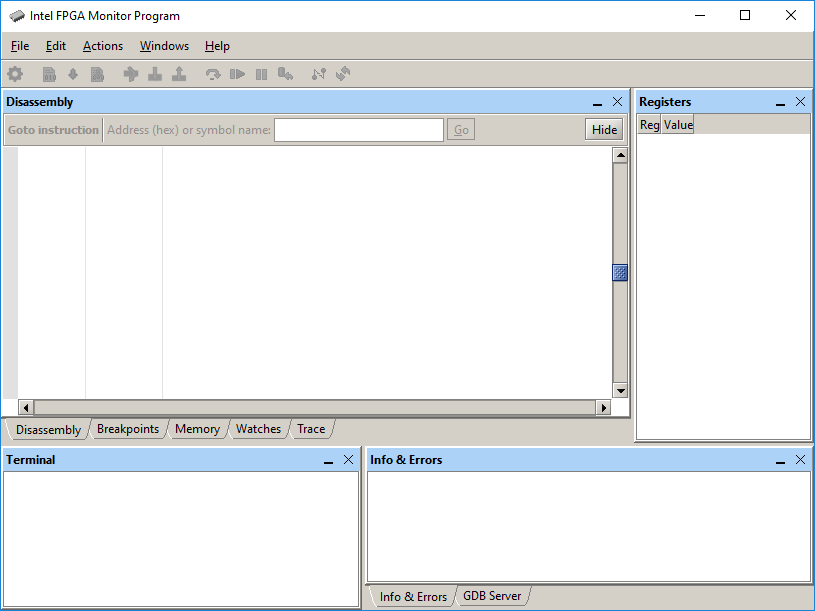
\includegraphics[scale=.45]{figures/figureMP1.png}
	\end{center}
	\caption{The \productNameMed{} window.}
\label{fig:MP1}
\end{figure}

To develop Nios II software code using the Monitor Program it is necessary to create a new 
project.  Select {\sf File $>$ New Project} to reach the window in Figure~\ref{fig:MP2}.
Give the project a name and indicate the folder for the project; 
we have chosen the project name {\it lab1\_part1} in the folder {\it
Exercise1$\backslash$Part1}, as indicated in the figure. Use the drop-down menu 
shown in Figure~\ref{fig:MP2} to set the target architecture to the Nios II processor.
Click {\sf Next}, to get the window in Figure~\ref{fig:MP3}.

\begin{figure}[H]
	\begin{center}
	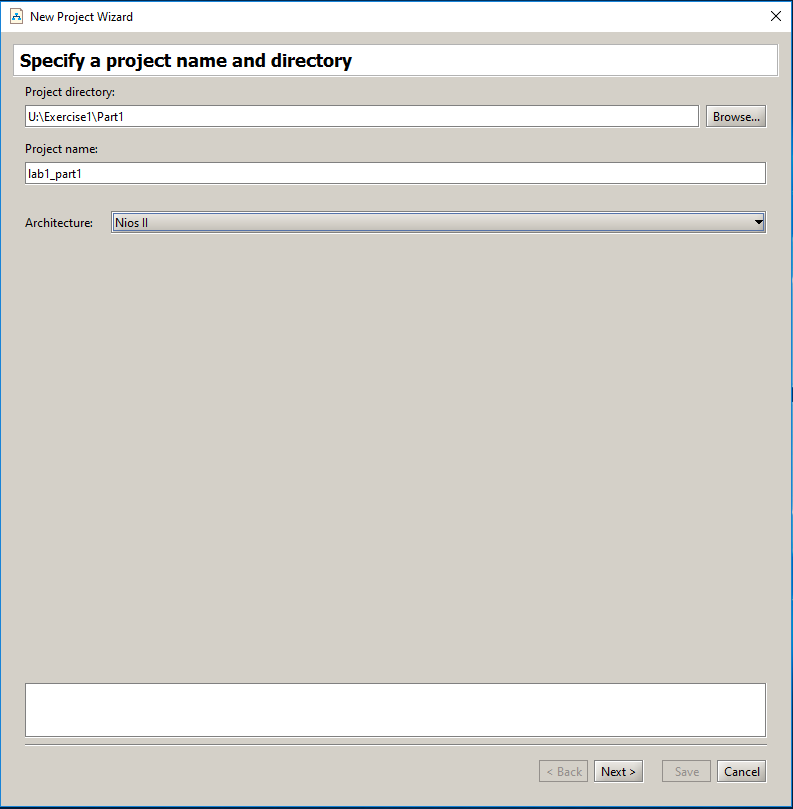
\includegraphics[scale=0.58]{figures/figureMP2.png}
	\end{center}
	\caption{Specify the folder and the name of the project.}
\label{fig:MP2}
\end{figure}

\begin{figure}[H]
	\begin{center}
	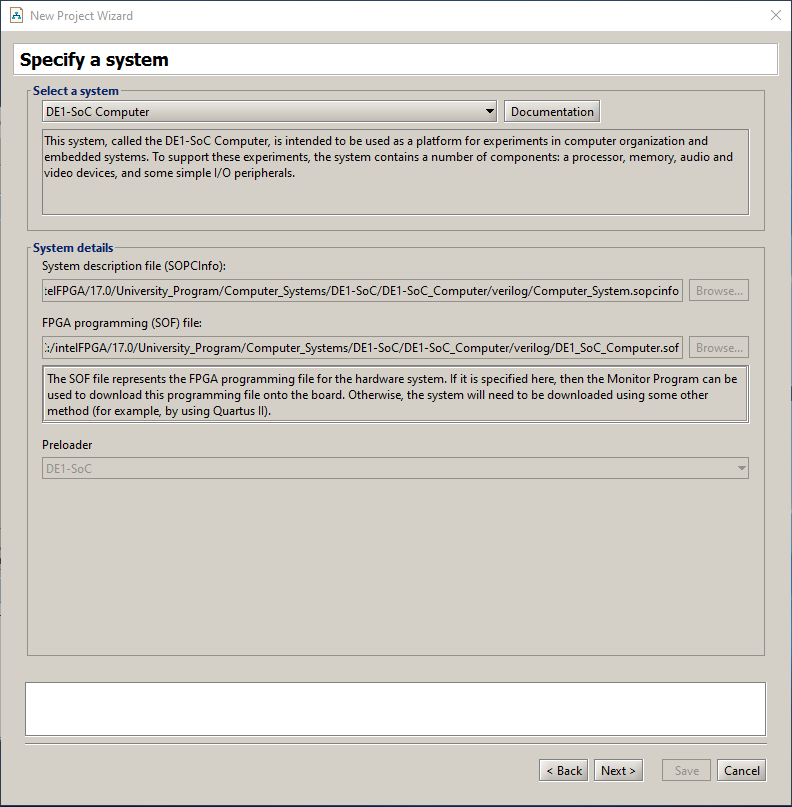
\includegraphics[scale=0.58]{figures/figureMP3.png}
	\end{center}
	\caption{Specification of the system.}
\label{fig:MP3}
\end{figure}

\item Now, you can select your own custom computer system (if you have one) or a 
pre-designed (by Intel) system. Choose the computer for your DE-series board listed in Table~\ref{tab:computer_systems}.  
The display in the window will now show where files that implement the pre-designed system are 
located. If you select a computer system that you designed yourself, then you have to 
provide the locations of the corresponding files. Click {\sf Next}.

\begin{table}[H]
	\begin{center}
	\begin{tabular}{ l | l }
	\bf{Board} & \bf{Computer System} \\
	\hline
	\rule{0pt}{3ex}DE0-CV & DE0-CV Computer \\ 
	DE1-SoC & DE1-SoC Computer \\
	DE2-115 & DE2-115 Computer \\
	DE10-Lite & DE10-Lite Computer \\
	DE10-Standard & DE10-Standard Computer \\
	\end{tabular}
	\caption{DE-series board computer systems}
	\label{tab:computer_systems}
	\end{center}
\end{table}

\item In the window in Figure~\ref{fig:MP4} you can specify the type of application 
programs that you wish to run. They can be written in either assembly language
or the C programming language.  Specify that an assembly language program will be used. 
The \productNameMed{} package contains several sample programs.
Select the box {\sf Include a sample program with the project}.
Then, choose the {\sf Getting Started} program, as indicated in the figure, and 
click {\sf Next}.

\begin{figure}[H]
	\begin{center}
	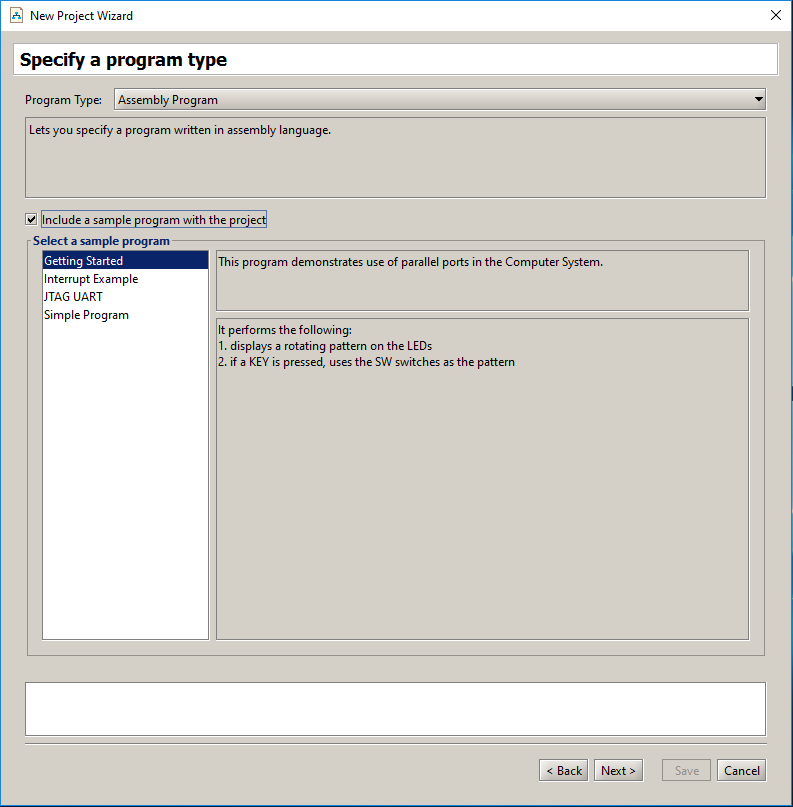
\includegraphics[scale=0.50]{figures/figureMP4.png}
	\end{center}
	\caption{Selection of an application program.}
\label{fig:MP4}
\end{figure}

\item The window in Figure~\ref{fig:MP5} is used to specify the source file(s) that contain the
application program(s). Since we have selected the {\it Getting Started} program, the window indicates the source
code file for this program. This window also allows the user to specify the starting point in the
selected application program. The default symbol is {\it \_start}, which is used
in the selected sample program. Click {\sf Next}.

\begin{figure}[H]
	\begin{center}
	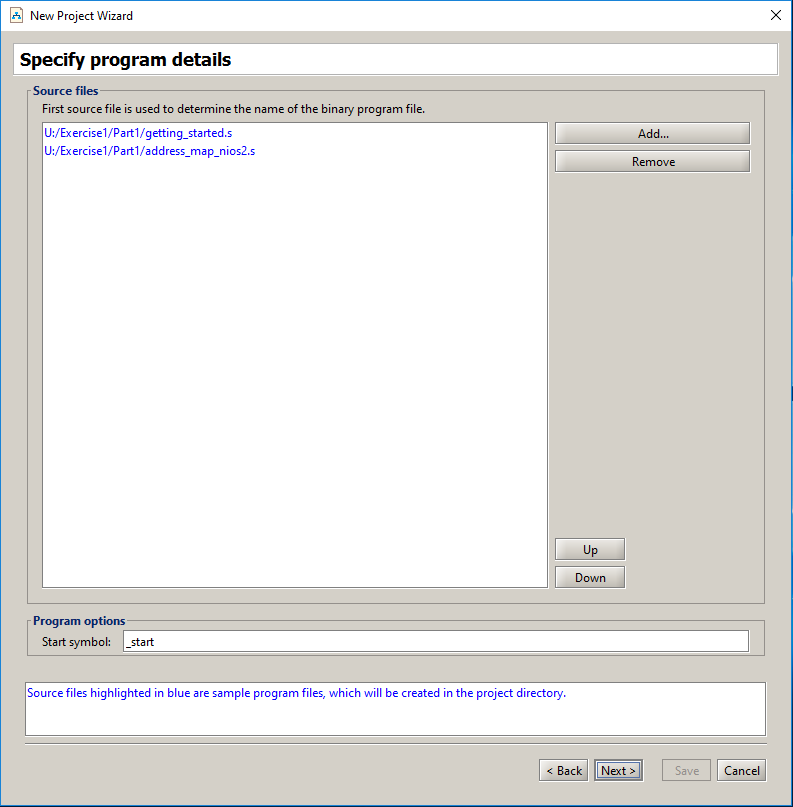
\includegraphics[scale=0.50]{figures/figureMP5.png}
	\end{center}
	\caption{Source files used by the application program.}
\label{fig:MP5}
\end{figure}

\item The window in Figure~\ref{fig:MP6} indicates some system parameters.
Note that the figure indicates that the {\it DE-SoC [USB-1]} cable is selected to provide 
the connection between the DE1-SoC board and the host computer. This is the name assigned to the 
USB-Blaster connection between the computer and the DE1-SoC board.
For some boards, the connection may be called {\it USB-Blaster [USB-0]}.  Click {\sf Next}.

\begin{figure}[H]
	\begin{center}
	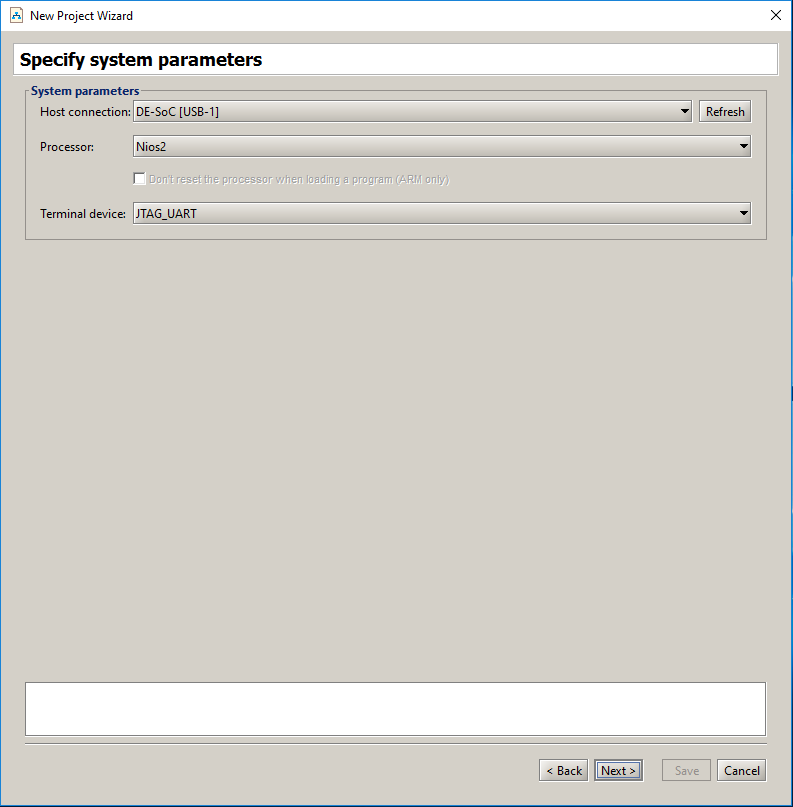
\includegraphics[scale=0.58]{figures/figureMP6.png}
	\end{center}
	\caption{Specify the system parameters.}
\label{fig:MP6}
\end{figure}

\item The window in Figure~\ref{fig:MP7} displays the names of Assembly sections that will
be used for the program, and allows the user to select a target memory location
for each section. In this case only the .{\it text} section, which corresponds to
the program code (and data), is defined. As shown in the figure, the .{\it text}
section is targeted to the SDRAM memory in the Computer, starting at
address 0. Click {\sf Finish} to complete the specification of the new project.

\begin{figure}[H]
	\begin{center}
	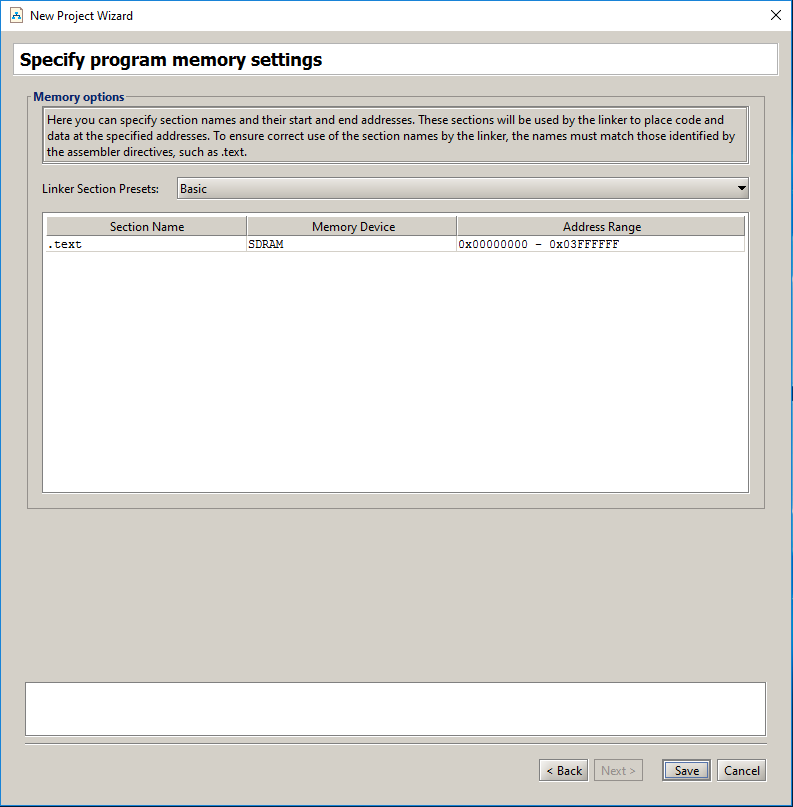
\includegraphics[scale=0.58]{figures/figureMP7.png}
	\end{center}
	\caption{Specify the program memory settings.}
\label{fig:MP7}
\end{figure}

\item Since you specified a new project, a pop-up box will appear asking if
you want to download the system associated with this project onto your DE-series board.
Make sure that the power to the board is turned on and click {\sf Yes}.
After the download is complete, a pop-up box
will appear informing you that the circuit has been successfully downloaded. Click {\sf OK}.
If the circuit is not successfully downloaded, make sure that the USB connection, through 
which the USB-Blaster communicates, is established and recognized by the host computer. 
(If there is a problem, a possible
remedy may be to unplug the USB cable and then plug it back in.)
\item Having downloaded the Computer into the FPGA on your DE-series board, 
we can now load and run the sample program.
In the main Monitor Program window, shown in Figure~\ref{fig:MP9}, 
select {\sf Actions $>$ Compile \& Load} 
to assemble the Nios II program and then load it into the FPGA chip.
Figure~\ref{fig:MP9} shows the Monitor Program window after the sample program has been loaded. 
\item Run the program by selecting {\sf Actions $>$ Continue} or
by clicking on the toolbar icon \hbox{
\includegraphics[scale=0.8]{figures/icon_continue.png}}, 
and observe the patterns displayed on the LEDs and 7-segment displays. 
\item Pause the execution of the sample program by clicking on the 
icon \hbox{
\includegraphics[scale=0.8]{figures/icon_pause.png}}, 
and disconnect from this session
by clicking on the icon \hbox{
\includegraphics[scale=0.8]{figures/icon_disconn.png}}, 

\begin{figure}[H]
	\begin{center}
	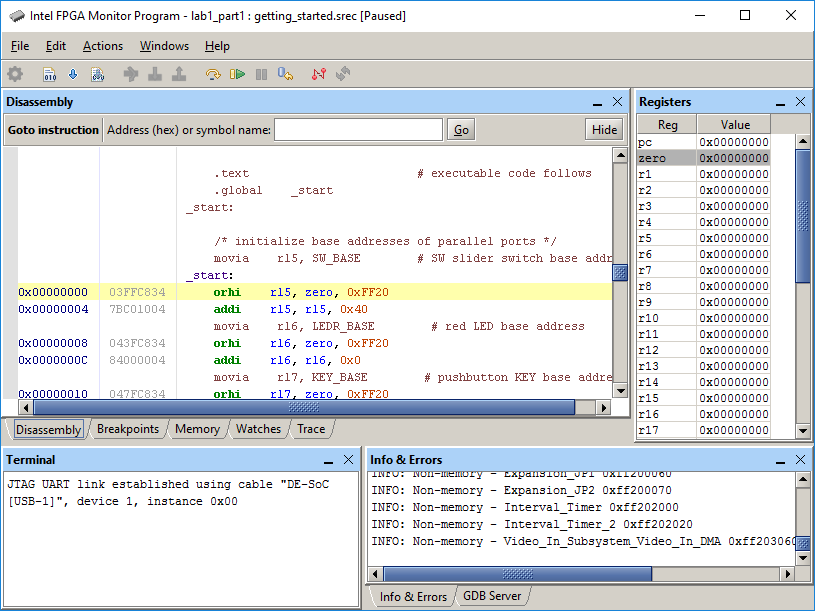
\includegraphics[scale=0.58]{figures/figureMP9.png}
	\end{center}
	\caption{The monitor window showing the loaded sample program.}
\label{fig:MP9}
\end{figure}

\end{enumerate}

\clearpage

\section*{Part II}
\addcontentsline{toc}{2}{Part II}
Now, we will explore some features of the Monitor Program by using a
simple application program written in the Nios II assembly language.
Consider the program in Figure~\ref{fig:code}, which finds the largest number in a list
of 32-bit integers that is stored in the memory.

\begin{figure}[H]
\begin{center}
\lstinputlisting[style=defaultNiosStyle]{../design_files/part2.s}
\end{center}
\caption{Assembly-language program that finds the largest number.}
\label{fig:code}
\end{figure}

Note that some sample data is included in this program.
The word (4 bytes) at the label {\it RESULT} is reserved for storing the result, which will be 
the largest number found. The next word, $N$, specifies the number of entries in the list.
The words that follow give the actual numbers in the list.

~\\
Make sure that you understand the program in Figure~\ref{fig:code} and the meaning of each 
instruction in it. Note the extensive use of comments in the program.
You should always include meaningful comments in programs that you will write!

Perform the following:

\begin{enumerate}
\item Create a new folder for this part of the exercise, with a name such as {\it Part2}.  
Create a file named {\it part2.s} and enter the code from Figure~\ref{fig:code} into this
file.  Use the Monitor Program to create a new project in this folder; we have chosen the 
project name {\it part2}.  When you reach the window in Figure~\ref{fig:MP4} 
choose {\sf Assembly Program} but do not select a sample program. Click {\sf Next}.
\item Upon reaching the window in Figure~\ref{fig:MP5}, you have to specify the source
		  code file for your program.
Click {\sf Add} and in the pop-up box that appears indicate the desired file name,
{\it part2.s}.  Click {\sf Next} to get to the window in Figure~\ref{fig:MP6}. 
Again click {\sf Next} to get to the window in Figure~\ref{fig:MP7}. Notice that the 
SDRAM is selected as the memory device.  Your program will be loaded starting at
address 0 in this memory.  Click {\sf Finish}.
\item Compile and load the program.

\item The Monitor Program will display a disassembled view of the machine code loaded
		  in the memory, as indicated in Figure~\ref{fig:MP11}. 
Note that the pseudo instruction {\bf movia r8, RESULT} from your source code
has been implemented by using the two instructions {\bf orhi r8, zero, 0x0} and 
{\bf addi r8, r8, 0x38}.  These instructions load the 32-bit address of the label RESULT,
which is {\sf 0x00000038}, into register r8.

\begin{figure}[H]
	\begin{center}
	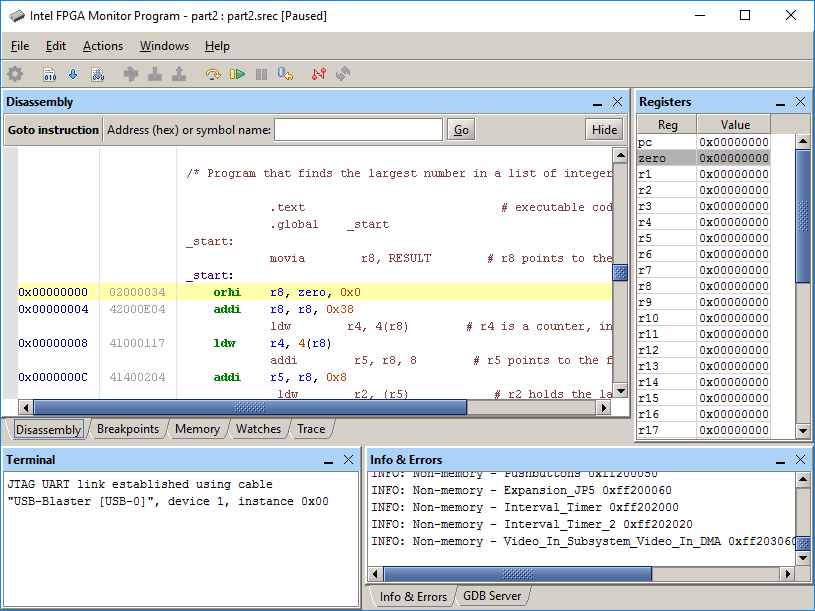
\includegraphics[scale=0.58]{figures/figureMP11.png}
	\end{center}
	\caption{The disassembled view of the program in Figure~\ref{fig:code}.}
\label{fig:MP11}
\end{figure}

\newpage
\item Execute the program. When the code is running, you will not be able to see any changes
(such as the contents of registers or memory locations) in the Monitor Program windows,
because the Monitor Program cannot communicate with the computer while code is being
executed.  But, if you pause the program then the Monitor Program windows will be updated.
Pause the program using the icon \hbox{
\includegraphics[scale=0.8]{figures/icon_pause.png}}
and observe that the processor stops within the endless loop {\bf STOP: br STOP}.
Note that the largest number found in the sample list is 8 as indicated
by the content of register r2. This result is also stored in memory at the label
RESULT.  As discussed above, the address of the label RESULT for this program is {\sf 0x00000038}.
Use the Monitor Program's Memory tab, as illustrated in Figure~\ref{fig:MP_mem},
to verify that the resulting value 8 is stored in the correct location.
\item You can return control of the program to the start by clicking 
		  on the icon \hbox{
\includegraphics[scale=0.8]{figures/icon_restart.png}}, or by
		  selecting {\sf Actions} $>$ {\sf Restart}. 
Do this and then single-step through the program by clicking on the icon
\hbox{
\includegraphics[scale=0.8]{figures/icon_step.png}}. Watch how the instructions change the 
data in the processor's registers. 


\item Double-click on the {\sf pc} register in the Monitor Program and then set the program
		  counter to 0. Note that this action has the same effect as
clicking on the restart icon \hbox{
\includegraphics[scale=0.8]{figures/icon_restart.png}}. 
\item Now set a breakpoint at address {\sf 0x0000002C} (by clicking on the gray bar to
the left of this address), so that the program will 
automatically stop executing whenever the branch instruction at this location is about to
be executed. Restart the program and run it again.  Observe the contents of register r2 each time
the breakpoint is reached.

\end{enumerate}

\begin{figure}[h]
	\begin{center}
	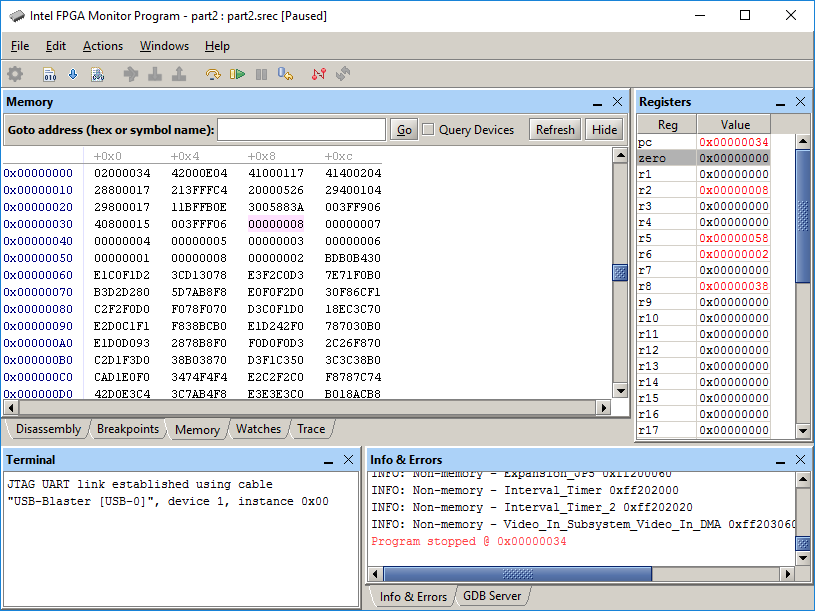
\includegraphics[scale=0.58]{figures/figureMP_mem.png}
	\end{center}
	\vspace{-0.5cm}\caption{Displaying the result in the memory tab.}
\label{fig:MP_mem}
\end{figure}

\newpage

\section*{Part III}
\addcontentsline{toc}{3}{Part III}
Implement the task in Part II by modifying the program in Figure~\ref{fig:code} so that it
uses a subroutine. The subroutine, LARGE, has to find the largest number in a list.
The main program passes the number of entries and the address of the start of the
list as parameters to the subroutine via registers r4 and r5.
The subroutine returns the value of the largest number to the calling program
via register r2. A suitable main program is given in Figure~\ref{fig:main}.
~\\


Create a new folder and a new Monitor Program project to compile and download your program.
Run your program to verify its correctness.

\begin{figure}[H]
\begin{center}
\lstinputlisting[style=defaultNiosStyle]{../design_files/part3.s}
\end{center}
\caption{Main program for Part III.}
\label{fig:main}
\end{figure}


\section*{Part IV}
\addcontentsline{toc}{4}{Part IV}
The program shown in Figure~\ref{fig:decimal} converts a binary number to two decimal digits.
The binary number is loaded from memory at the location $N$, and the two
decimal digits that are extracted from $N$ are stored into memory in two bytes starting at 
the location {\it Digits}. For the value $N = 76$ ({\sf0x4c}) shown in the figure, the code sets 
{\it Digits} to {\sf 00000706}.

~\\

Make sure that you understand how the code in Figure~\ref{fig:decimal} works. Then, extend
the code so that it converts the binary number to four decimal digits, supporting decimal 
values up to 9999. You should modify the DIVIDE subroutine so that it can use any divisor, 
rather than only a divisor of 10. Pass the divisor to the subroutine in register r5.

~\\

If you run your code with the value $N = 9876$ ({\sf0x2694}), then {\it Digits} should be set to 
{\sf 09080706}.

\begin{figure}[H]
\begin{center}
\lstinputlisting[style=defaultNiosStyle]{../design_files/part4.s}
\end{center}
\caption{A program that converts a binary number to two decimal digits.}
\label{fig:decimal}
\end{figure}


%%%%%%%%%%%%%%%%%%%%%%%%%%%%%%%%%%%%%%%%
%%% FPGAcademy Copyright Information %%%
%%%%%%%%%%%%%%%%%%%%%%%%%%%%%%%%%%%%%%%%

%Always put the copyright on a new page (clear page), with some vertical space from top
\clearpage
\vspace{1in}

\noindent

Copyright {\copyright} FPGAcademy.org. All rights reserved. FPGAcademy and the 
FPGAcademy logo are trademarks of FPGAcademy.org.  This document is provided 
"as is", without warranty of any kind, express or implied, including but not 
limited to the warranties of merchantability, fitness for a particular purpose 
and noninfringement. In no event shall the authors or copyright holders be 
liable for any claim, damages or other liability, whether in an action of 
contract, tort or otherwise, arising from, out of or in connection with the 
document or the use or other dealings in the document.
~\\
~\\
**Other names and brands may be claimed as the property of others.


\end{document}
